\documentclass[letterpaper,10pt]{article}
\usepackage{graphicx}
\usepackage{listings}
\usepackage{fullpage}
\usepackage{fixltx2e}
\usepackage{multirow}
\usepackage{amssymb,amsmath}
\usepackage{mathtools}
\usepackage[hyperfootnotes=false]{hyperref}
\usepackage{url}
\usepackage{subfig}
\usepackage{relsize}
\usepackage{enumitem}
\usepackage{fancyhdr}
\usepackage{framed}
\setlength{\headheight}{14pt}
\pagestyle{fancy}
\headsep = 20pt

% Lineskip mods
\linespread{1.0}
\setlength{\parskip}{0.5\baselineskip}
\setlength{\parindent}{0pt}
\newlength\docparskip
\parskip=6pt
\setlength{\docparskip}{\parskip}
\renewcommand{\arraystretch}{1.085}
\usepackage{xcolor}
\lstset{basicstyle=\ttfamily,
  showstringspaces=false,
  commentstyle=\color{red},
  keywordstyle=\color{blue}
}
\begin{document}

\fancyhf{}
\fancyhead[L]{AME 60614: Numerical Methods}
\fancyhead[R]{Qihao Zhuo: Problem Set 0}
\fancyfoot[C]{\thepage}

\thispagestyle{plain}
\begin{center}
  \large
  \textbf{AME 60614: Numerical Methods} \\
  \textbf{Fall 2021} \\
  \vspace{0.5em}
  \textbf{Problem Set 0} \\
  \vspace{1em}
  Qihao Zhuo
\end{center}

\vspace{1.5em}

\section{Code Documentation}

\begin{enumerate}
\item Download the document \texttt{sample\_ps0.tex} and \texttt{sample\_figure.eps} from the course Sakai page. Rename the file \texttt{lastname\_firstname\_ps0.tex}, and edit the report to add your name. Compile it using \texttt{pdflatex} or the \LaTeX\ editor of your choice.
  
\item Document your response to Problem 2 in your report. Use appropriately highlighted code listings for codes requested in Problem 2. Print a copy and bring it to class on the due date.
\end{enumerate}

\section{Computing in Parallel}
\subsection{Assignment}
\subsubsection{a}\label{sec21a}
The scripting language used is Matlab and the script is shown below. The sentences of plot or file 
can be commented out if there is no need for plot or output file. 
{\small\begin{framed}
  \begin{lstlisting}[language=Matlab]
    clear
    clc
    tic
    nx=10000;
    ny=10000;
    dx=2.5/(nx-1);
    dy=4.0/(ny-1);
    Re_plot = -2:dx:0.5;
    Im_plot = -2:dy:2;

    hold on

    f1 = fopen('exp.txt','w');
    for Re = Re_plot
        for Im = Im_plot
            c_p = Re + Im*1i;
            if(ms_check(c_p, 10))
                plot(Re, Im, 'r.');
                fprintf(f1,'%6.2f %6.2f\n',real(c_p),imag(c_p));
            end
        end
    end
    fclose(f1);
    toc

    function [logi] = ms_check(c, niter)
    z=0;
    count=0;
    while abs(z) < 2 && count < niter
        z = z^2 + c;
        count=count+1;
    end
    if count == niter
        logi=true;
    else
        logi=false;
    end
    end
    \end{lstlisting}
\end{framed}}

Fig.~\ref{figMat} is plotted by Matlab with a lower resolution. 
\begin{figure}[h]
  \centering
  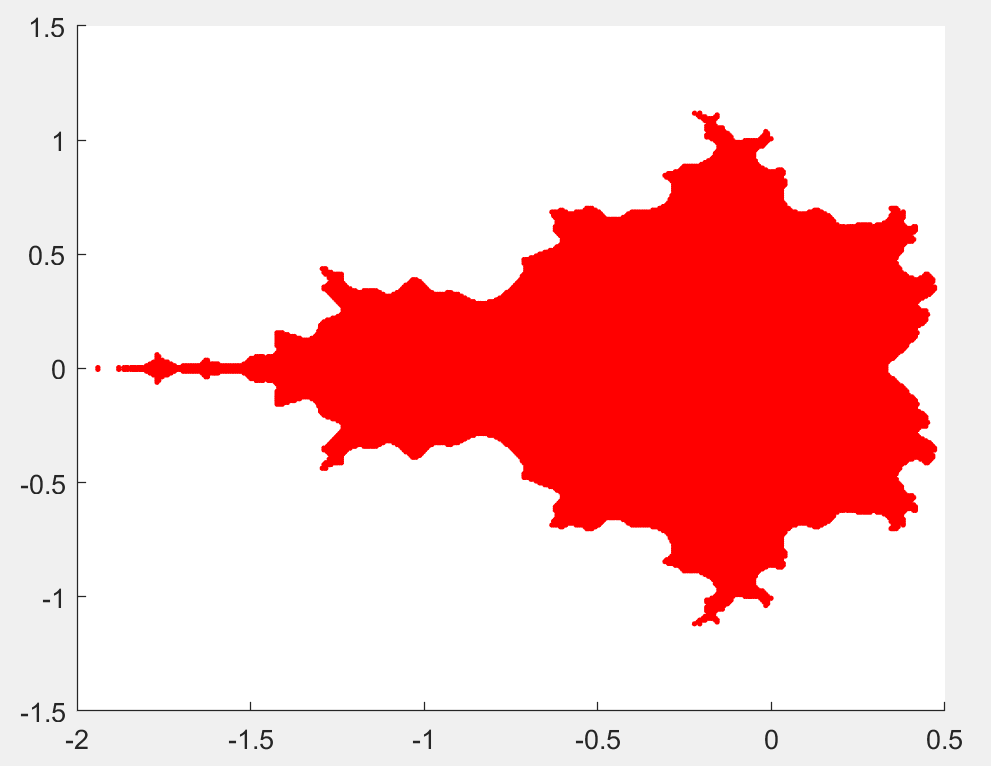
\includegraphics[width=0.5\textwidth]{FigMatlab.png}
  \caption{Figure of Mandelbrot Set by Matlab}
  \label{figMat}
\end{figure}

Since compiled language usually could not plot, Tab.~\ref{tabComMat} shows the time cost 
of Matlab scripts under $niter = 10,100,1000$ and will be compared with results of compiled language 
in Sec.~\ref{sec21b}.
\begin{table}
\centering
\caption{Time cost of Matlab while only writing output file}\label{tabComMat}
\begin{tabular}{cccc}
  \hline
  niter & 10 & 100 & 1000 \\
  \hline
  time & 524.60 & 501.68 & 927.91 \\
  \hline
\end{tabular}
\end{table}

The decrease between $niter = 10$ and $niter = 100$ might because when $niter = 10$, 
the number of points written to the output file is much more than $niter = 100$. The I/O operation would 
take a lot of time. 

\subsubsection{b}\label{sec21b}
Since in Fortran there is intrinsic $complex$ data type, the compile language used is Fortran. 
To compare with results in Sec.~\ref{sec21a}, I also let the Fortran program write the output file directly. 
The comparison of time cost is shown in Tab.~\ref{tabComMF}.
\begin{table}
\centering  
\caption{Comparison of time cost between Matlab and Fortran while only run iterations}\label{tabComMF}
\begin{tabular}{cccc}
  \hline
  niter & 10 & 100 & 1000 \\
  \hline
  Matlab & 524.60 & 501.68 & 927.91 \\
  Fortran & 44.21 & 53.61 & 235.97 \\
  \hline
\end{tabular}
\end{table}

Obviously Fortran performs better than Matlab. And in fact the Fortran can also write output file on 
my laptop, even for the 10000x10000 grid. Therefore compiled languages are much advantageous in such 
loops than scripting languages. The code used in this section is shown below. 
{\small\begin{framed}
  \begin{lstlisting}
    program MSet
        implicit none
        COMPLEX(kind=8) :: c,z
        REAL(kind=8) :: xmin,xmax,ymin,ymax,dx,dy
        INTEGER(kind=8) :: nx,ny,niter,i
        INTEGER(kind=8) :: cx,cy
        REAL(kind=8) :: t_begin,t_end

        OPEN(unit=1,file='MSet.in')
        READ(1,*) xmin,xmax,nx,ymin,ymax,ny,niter
        dx = (xmax-xmin)/(nx-1)
        dy = (ymax-ymin)/(ny-1)
        c = complex(xmin,ymin)
        OPEN(unit=2,file='dyIntMSet.out')
        CALL cpu_time(t_begin)
        do cx=1,nx-1
            do cy=1,ny-1
                z = (0,0)
                i = 1
                do while (abs(z)<=2 .AND. i<=niter)
                    z = z**2 + c
                    i = i + 1
                end do
                if ( i >= niter ) then
                  WRITE(2,*) real(c), AIMAG(c)
                end if
                c = complex(real(c),ymin+cy*dy)
            end do
            c = complex(xmin+cx*dx,ymin)
        end do
        CALL cpu_time(t_end)
        WRITE(*,*) "time", t_end-t_begin, "case", xmin,xmax,nx,ymin,ymax,ny,niter
    end program MSet
    \end{lstlisting}
\end{framed}}

With points from the Fortran program, Fig.~\ref{figMS} is also a figure of the Mandelbrot set. 
\begin{figure}[h]
  \centering
  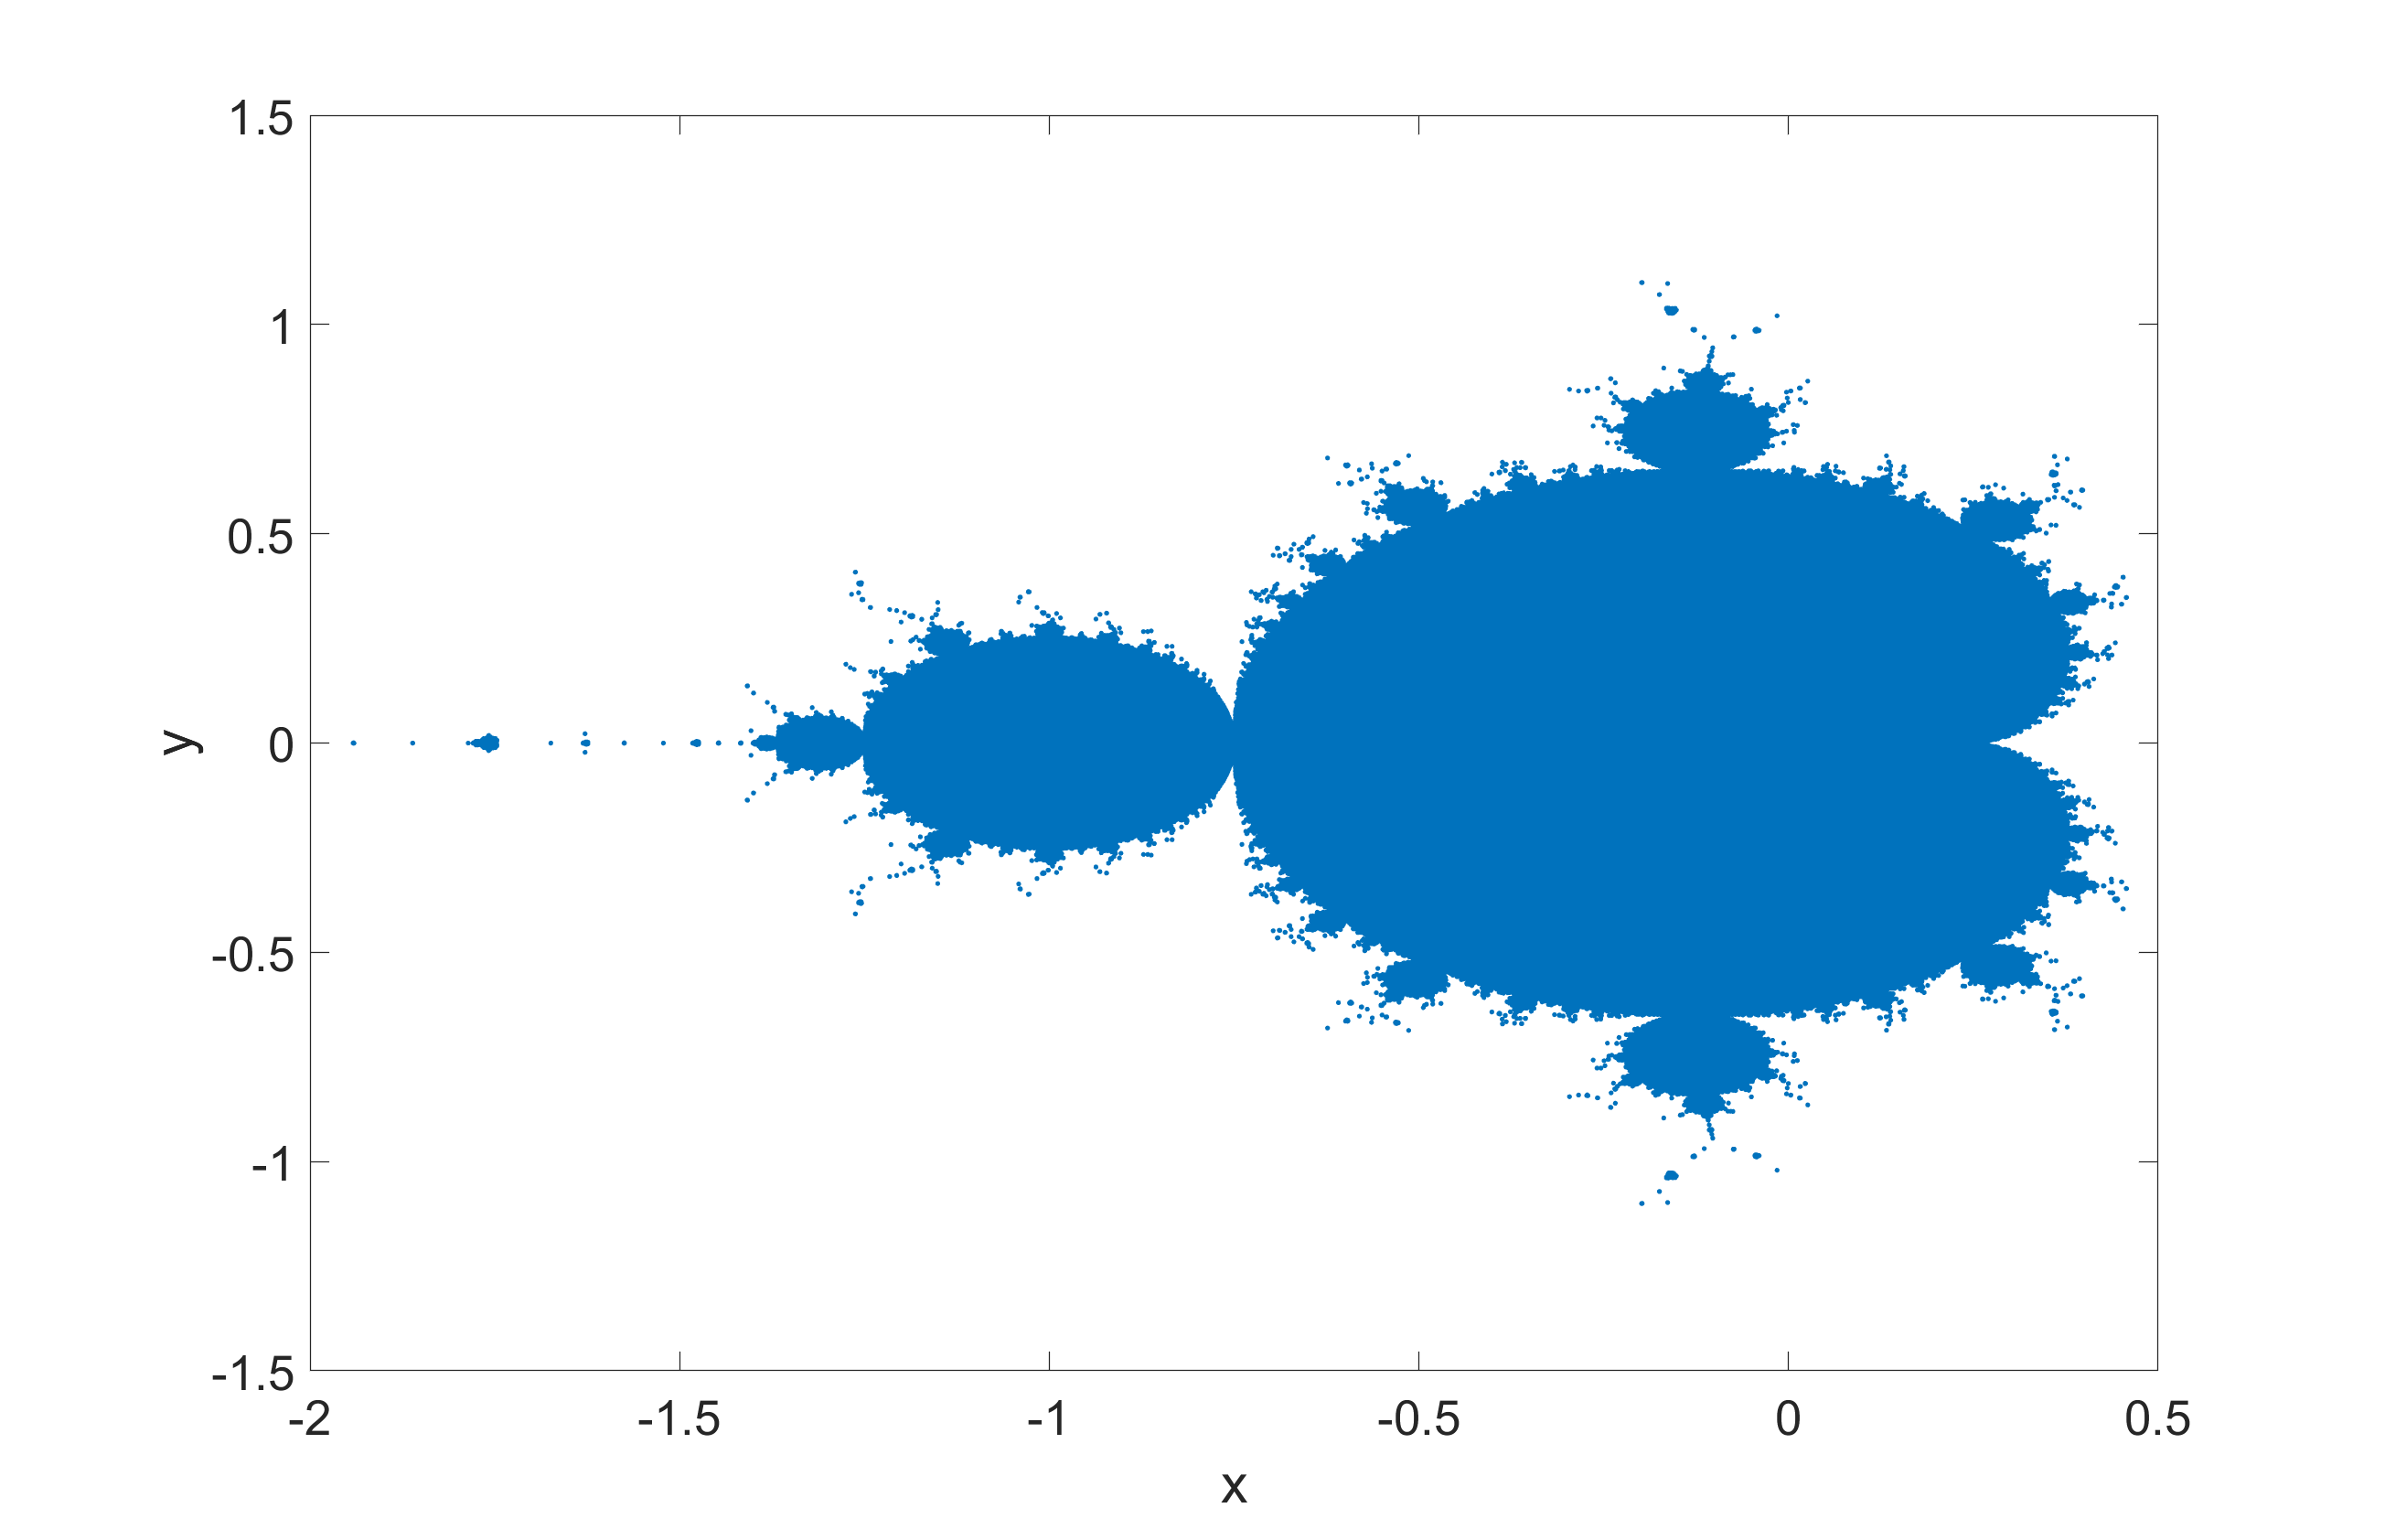
\includegraphics[width=0.5\textwidth]{F1_4.png}
  \caption{Figure of Mandelbrot Set by data from Fortran}
  \label{figMS}
\end{figure}

\subsubsection{c}\label{sec21c}
To plot the figure of Mandelbrot Set, there are three methods. The first is to write $c$ to the output file 
directly in each loop, which was used in Sec.~\ref{sec21b}. But it is low efficient because there are also 
too much I/O operation on the output file. 
The second is to record $c$ in an array and write all picked points to the output file 
at the end of code. The third is to record intergers indicating $c$ and compute corresponding $c$ 
when writing the outpu file. The comparison between timecost of them are shown in Tab.~\ref{tabComWr} with cases 
under 2 threads and 4 threads for $niter=1000$. 
\begin{table}
\centering
\caption{Comparison between different methods of output}\label{tabComWr}
\begin{tabular}{cccc}
  \hline
  Thread & Method 1 & Method 2 & Method 3 \\
  \hline
  2 & 91.29 & 91.80 & 86.90 \\
  4 & 60.21 & 53.97 & 52.83 \\
  \hline
\end{tabular}
\end{table}

So in that section, the third method was chosen. The code is shown below. 

{\small\begin{framed}
  \begin{lstlisting}
    program MSet
        use omp_lib
        implicit none
        COMPLEX(kind=8) :: c,z
        REAL(kind=8) :: xmin,xmax,ymin,ymax,dx,dy
        INTEGER(kind=8) :: nx,ny,niter,i
        INTEGER(kind=8) :: cx,cy,j,k
        REAL(kind=8) :: t_begin,t_end,t_middle
        integer(kind=8),dimension(:,:),allocatable :: MS

        t_begin = omp_get_wtime()
        allocate (MS (10000,10000))
        MS = 0
        OPEN(unit=1,file='MSet.in')
        READ(1,*) xmin,xmax,nx,ymin,ymax,ny,niter
        dx = (xmax-xmin)/(nx-1)
        dy = (ymax-ymin)/(ny-1)
        c = complex(xmin,ymin)
        OPEN(unit=2,file='Int.out')
        
        !$OMP PARALLEL DO SCHEDULE(guided) SHARED(MS) PRIVATE(cx,cy,i,c,z)
        do cx=1,nx-1
            do cy=1,ny-1
                z = (0,0)
                i = 1
                do while (abs(z)<=2 .AND. i<=niter)
                    z = z**2 + c
                    i = i + 1
                end do
                if ( i >= niter ) then
                    MS(cx,cy) = 1
                end if
                c = complex(real(c),ymin+cy*dy)
            end do
            c = complex(xmin+cx*dx,ymin)
        end do
        !$OMP END PARALLEL DO
        
        t_middle = omp_get_wtime()
        do j = 1, 10000
            do k = 1, 10000
                if ( MS(j,k) /= 0 ) then
                    WRITE(2,*) xmin+j*dx, ymin+k*dy
                end if
            end do
        end do
        t_end = omp_get_wtime()
        WRITE(*,*) "time", t_end-t_begin, t_middle-t_begin, t_end-t_middle
        WRITE(*,*) "case", xmin,xmax,nx,ymin,ymax,ny,niter 

    end program MSet
    \end{lstlisting}
\end{framed}}

My personal machine only has two cores and much low performance, so the parallel part was taken on 
a work station of our research group. So the serial performance in this section was re-computed and 
results are shown in Tab.~\ref{tabFS}. 

Adding the optimization option "-O3" when compiling the code, the computation will be speeded up, especially 
for higher threads. The comparison under $niter=1000$ is shown in Tab.~\ref{tabComO3}. 
\begin{table}
  \centering  
  \caption{Comparison between diffrent SCHEDULE under $niter=1000$}\label{tabComO3}
  \begin{tabular}{ccccccc}
    \hline
    Threads & 2 & 4 & 8 & 16 &32 &64\\
    \hline
    Without O3 & 139.89& 74.64& 46.93 &26.48&15.28&8.49\\
    With O3 & 68.278& 33.03& 17.22&9.01&6.25&3.90\\
    \hline
  \end{tabular}
\end{table}

By the way, it was also noticed that when parallel computing, the threads are not always working fully. From the Fig.~\ref{figMS}, 
the distribution of points in the Mandelbrot set is not uniform. So for different $c$, the actual number of iterations 
will be totally different. That might decrease the computation efficiency if the points of $s$ are allocated to threads 
equally and statically. It seems efficient enough that each thread handles same amount of $c$, but the actual workload 
will be different. 

A handle named SHCEDULE could be added to the PARALLEL sentence so that the distribution of tasks for each thread can be dynamic 
to keep all threads at work fully. For $niter = 1000$, the time cost comparison between static scheduel and guided scheduel 
is shown in Tab.~\ref{tabComSche}. 
\begin{table}
\centering  
\caption{Comparison between diffrent SCHEDULE under $niter=1000$}\label{tabComSche}
\begin{tabular}{ccccccc}
  \hline
  Threads & 2 & 4 & 8 & 16 &32 &64\\
  \hline
  Defaut SCHEDULE & 117.37& 61.08& 39.24&22.18&12.97&6.85\\
  Guided SCHEDULE & 68.278& 33.03& 17.22&9.01&6.25&3.90\\
  \hline
\end{tabular}
\end{table}

\subsubsection{d}
The comparison of serial performances between the compiled language Fortran and the scripting language Matlab 
is shown in Tab.~\ref{tabComMF} and Sec.~\ref{sec21b}. And it shows that for such huge loops, 
compiled languages have much higer efficiency than scripting languages. 
By the way, the serial performance of Fortran can be discussed more. Furthermore, I tested its performance 
under $niter= 10,100,200,250,500,400,600,750,800,1000$. The results are shown in Tab.~\ref{tabFS}. 
\begin{table}
\centering  
\caption{Results of serial performances of Fortran}\label{tabFS}
\begin{tabular}{ccccccccccc}
  \hline
  niter & 10 & 100 & 200 & 250&400 & 500 & 600 & 750 & 800&1000\\
  \hline
  $t_{total}$ & 30.26&35.16&47.23&53.49&71.78&83.94&96.16&114.45&120.66&145.45\\
  $t_{loop}$ & 3.79&16.13&28.42&34.60&53.07&65.32&77.54&95.89&102.06&126.48\\
  $t_{output}$ & 26.47&19.03&18.81&18.89&18.72&18.63&18.63&18.56&18.60&18.97\\
  \hline
\end{tabular}
\end{table}

$t_{total}=t_{end}-t_{begin}$ means the total time cost of the program. $t_{loop}=t_{middle}-t_{begin}$ 
means the time cost of the loop part, e.g. the parallel part in the code. $t_{output}=t_{end}-t_{middle}$ 
means the time cost of writing the output file. 

The $t_{output}$ decreases because when $niter$ is low, the points picked are much more. Then the time cost 
on output would be more. When $niter > 200$, $t_{output}$ becomes almost stable, which means the amount of 
picked points becomes almost stable. 

So $t_{loop}$ will describe the performance more accurately than $t_{total}$. As for serial performances, 
Fig.~\ref{figFS} shows the relation between $niter$ and $t_{loop}$. Since it is for single thread, the it 
shows a simple linear relation, the more work load, the more time cost. 
\begin{figure}[h]
  \centering
  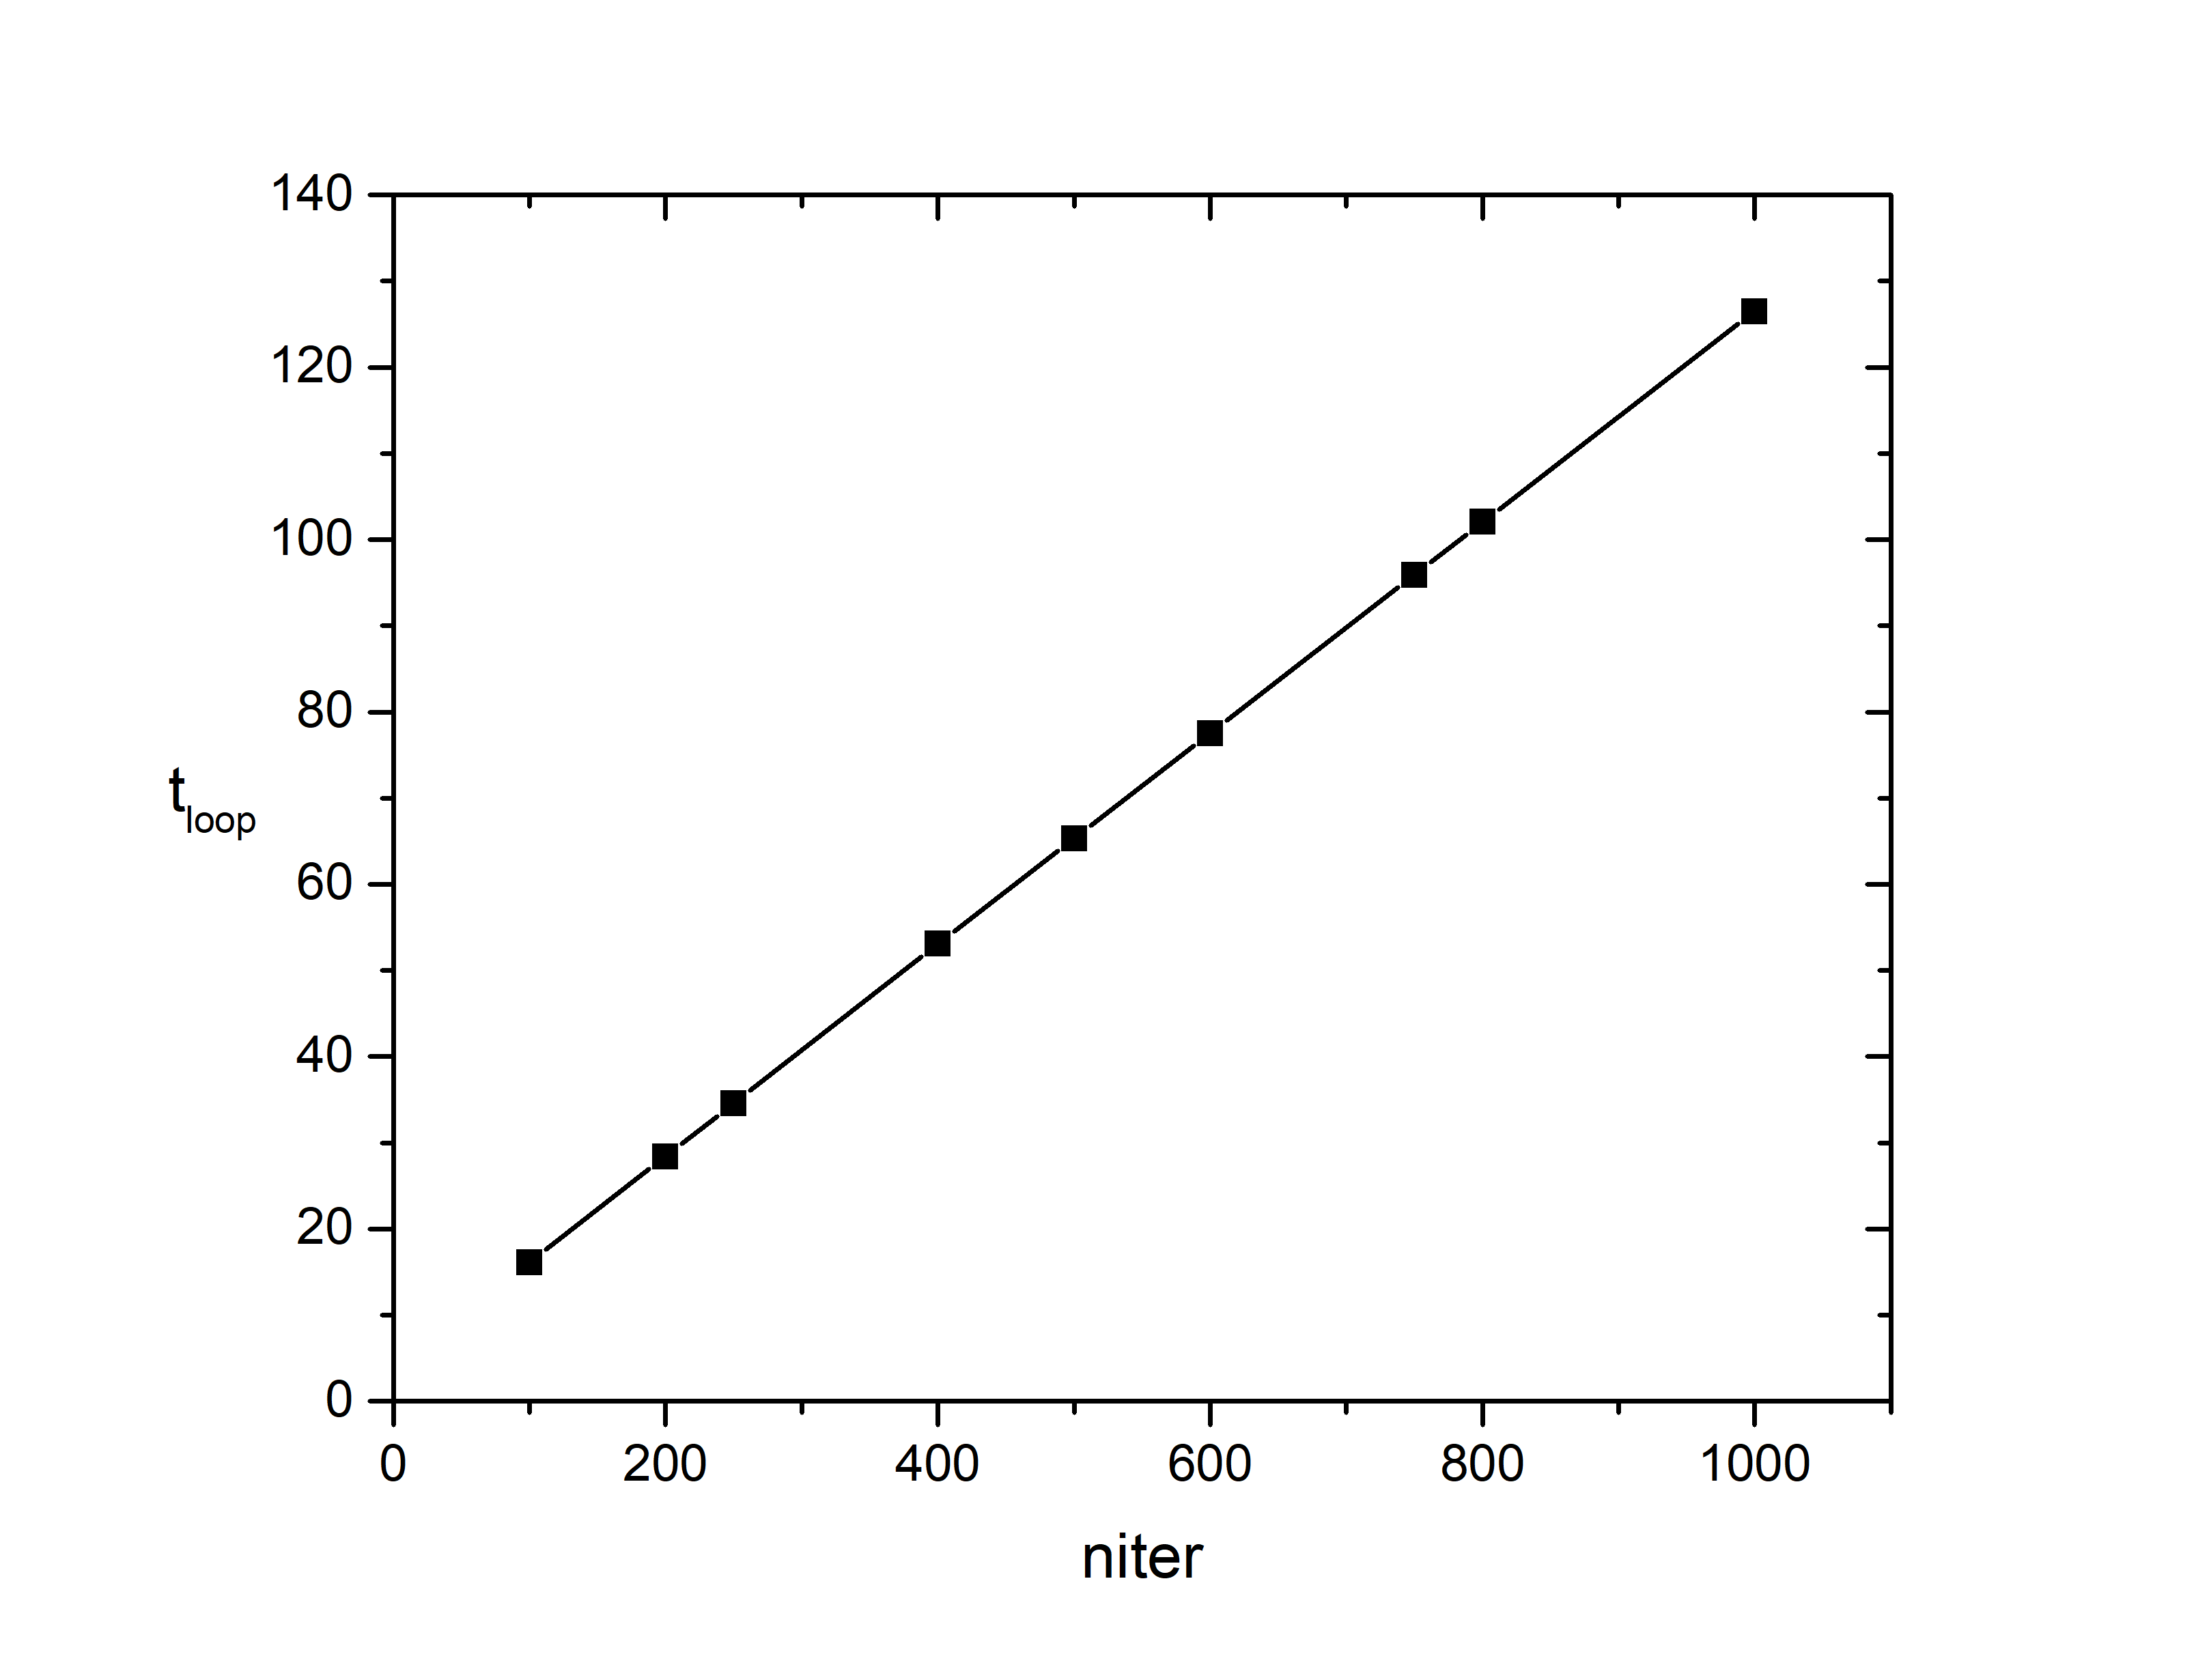
\includegraphics[width=0.5\textwidth]{figFS.png}
  \caption{Figure of $t_{loop}$ with niter}
  \label{figFS}
\end{figure}
In fact, when parallelizing the output part, which is also a DO LOOP, the time cost will increase much. 
I have not found the reason yet. 

I tested parallel performances with different number of threads to see the strong scaling speedup. 
Results of strong scaling speedup is shown in Fig.~\ref{figSS}. It shows that at the beginning of increasing 
threads, the performance increases linearly, but after about 10 threads, the increase becomes slower and slower. 
\begin{figure}[h]
  \centering
  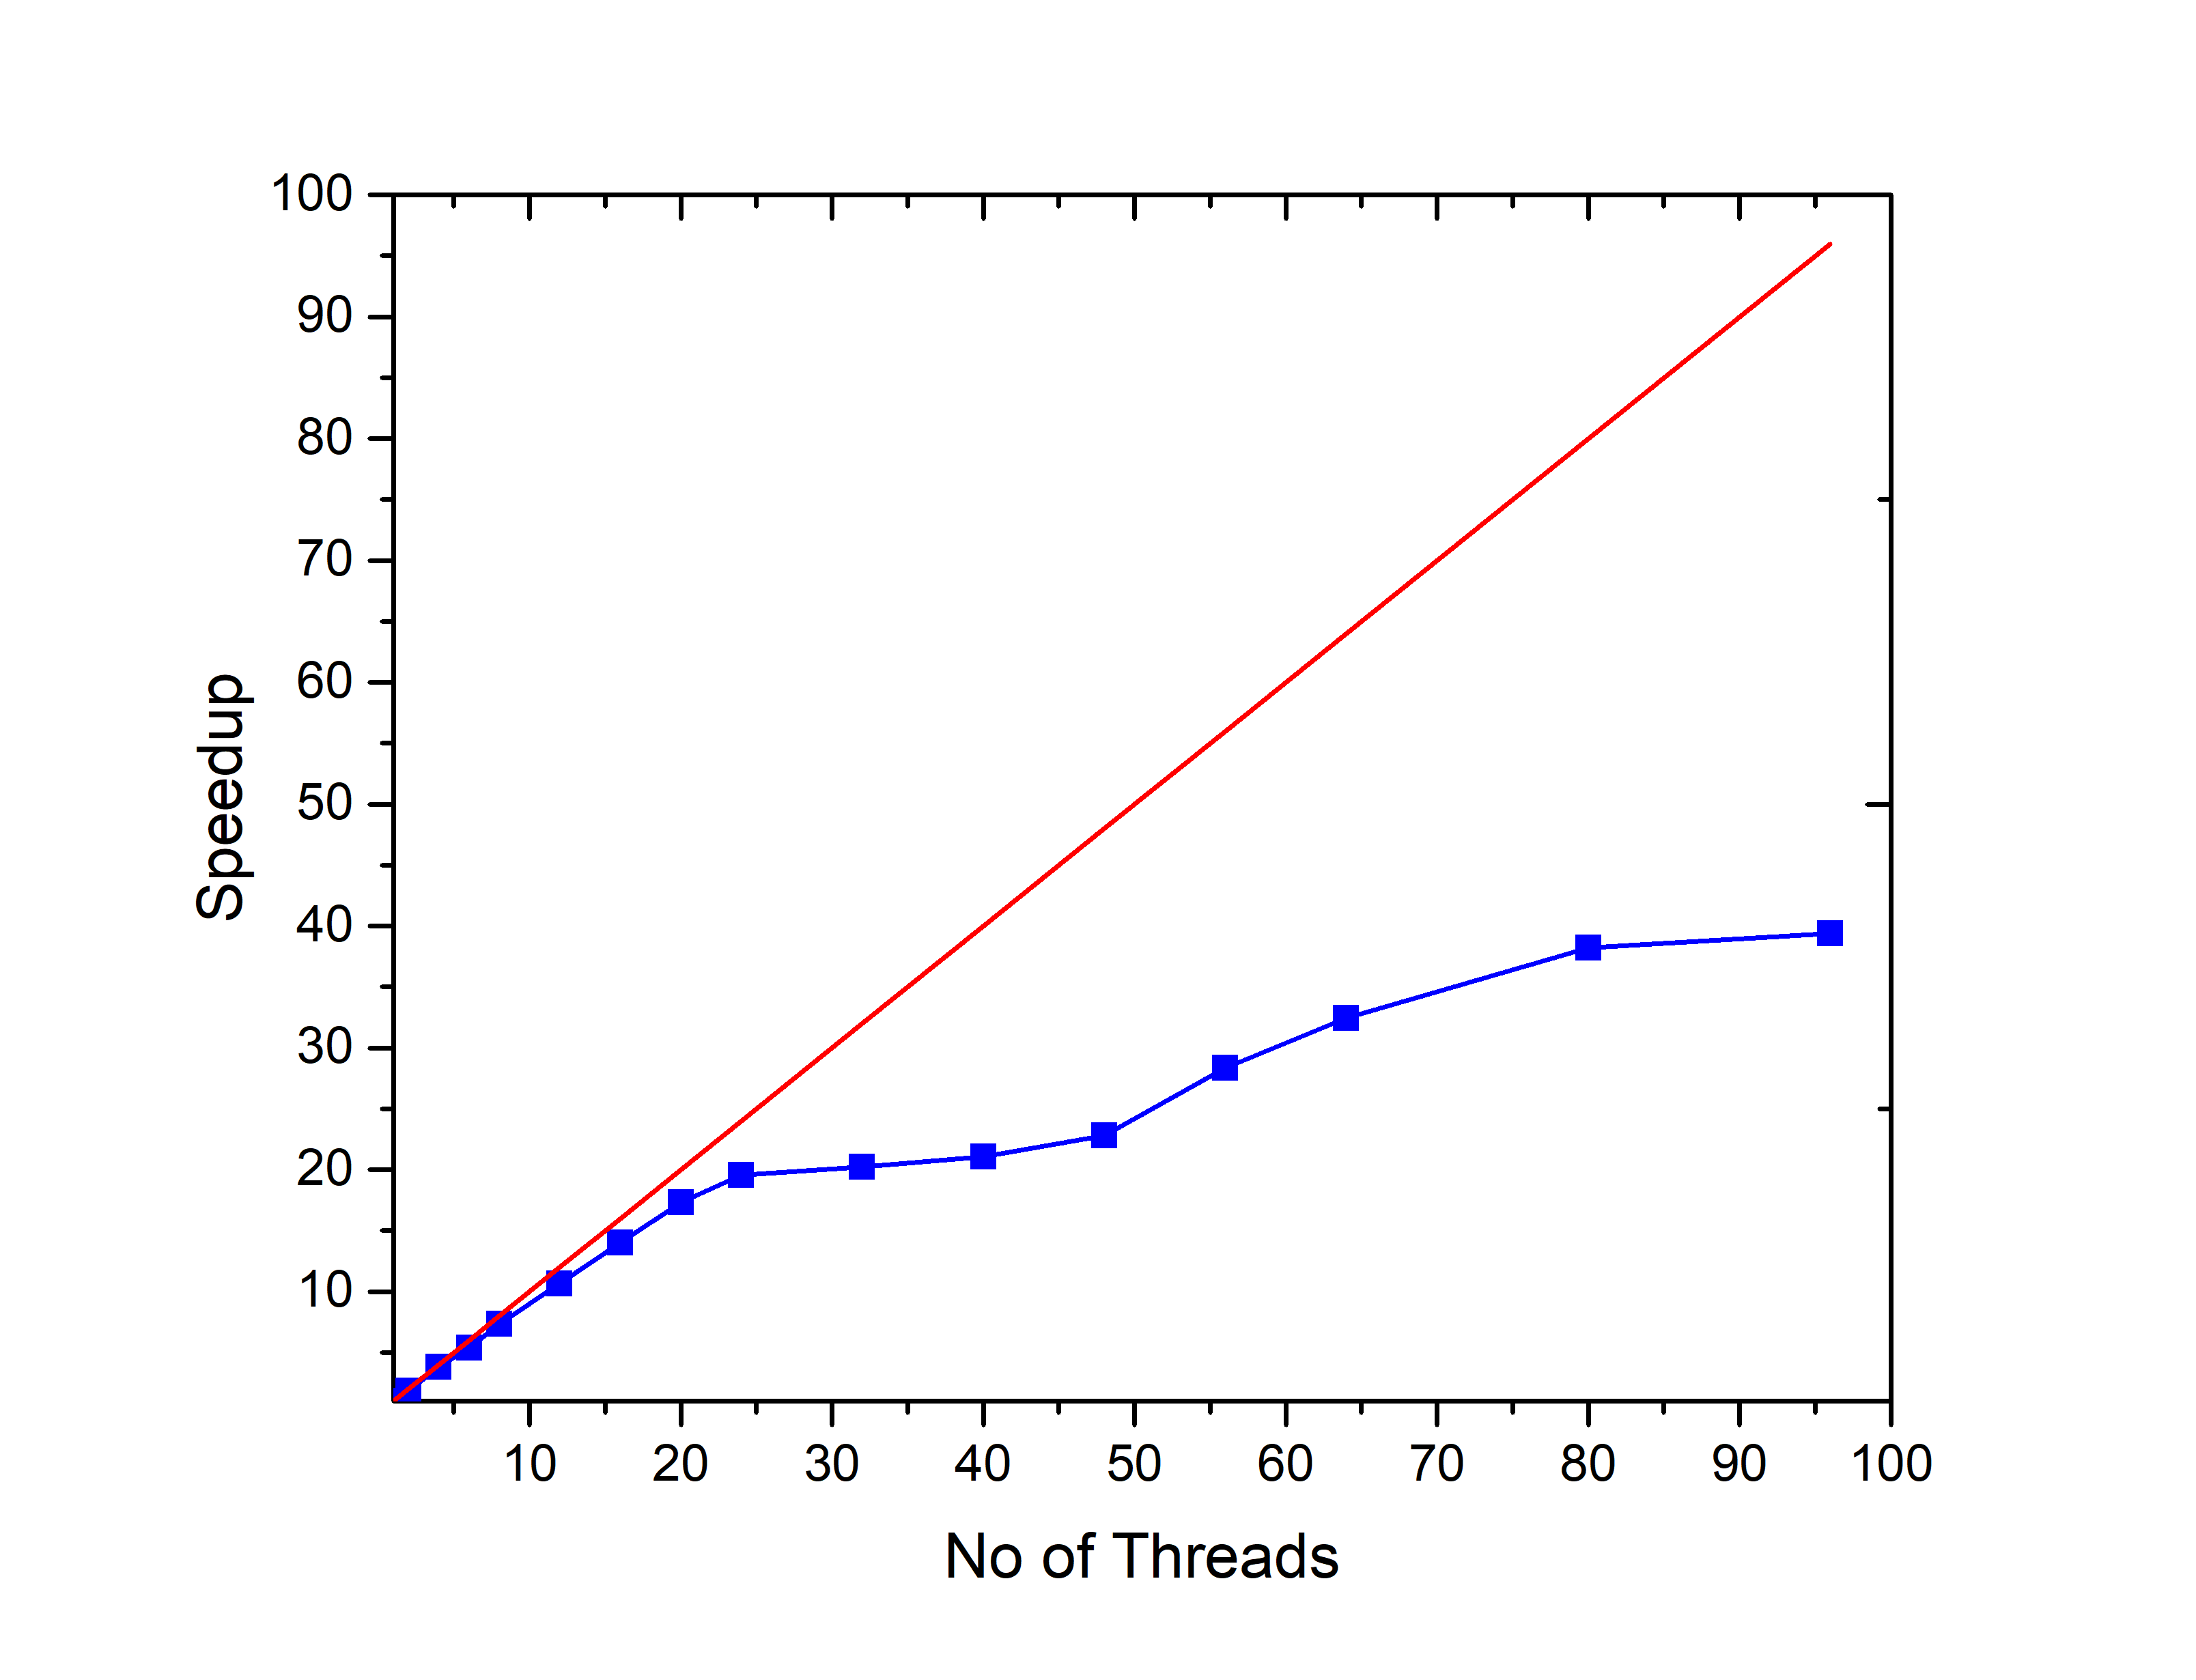
\includegraphics[width=0.5\textwidth]{StrongS.png}
  \caption{Figure of Strong Scaling}
  \label{figSS}
\end{figure}

Then I also tested the weak scaling efficiency. 
Results of weak scaling efficiency is shown in Fig.~\ref{figWS}. It shows that at the beginning of increasing 
threads, the efficiencies are close. I guess it is because the computation process is simple, then 
the efficiency can keep. But the efficieny decreases rapidly with increasing number of threads. 
\begin{figure}[h]
  \centering
  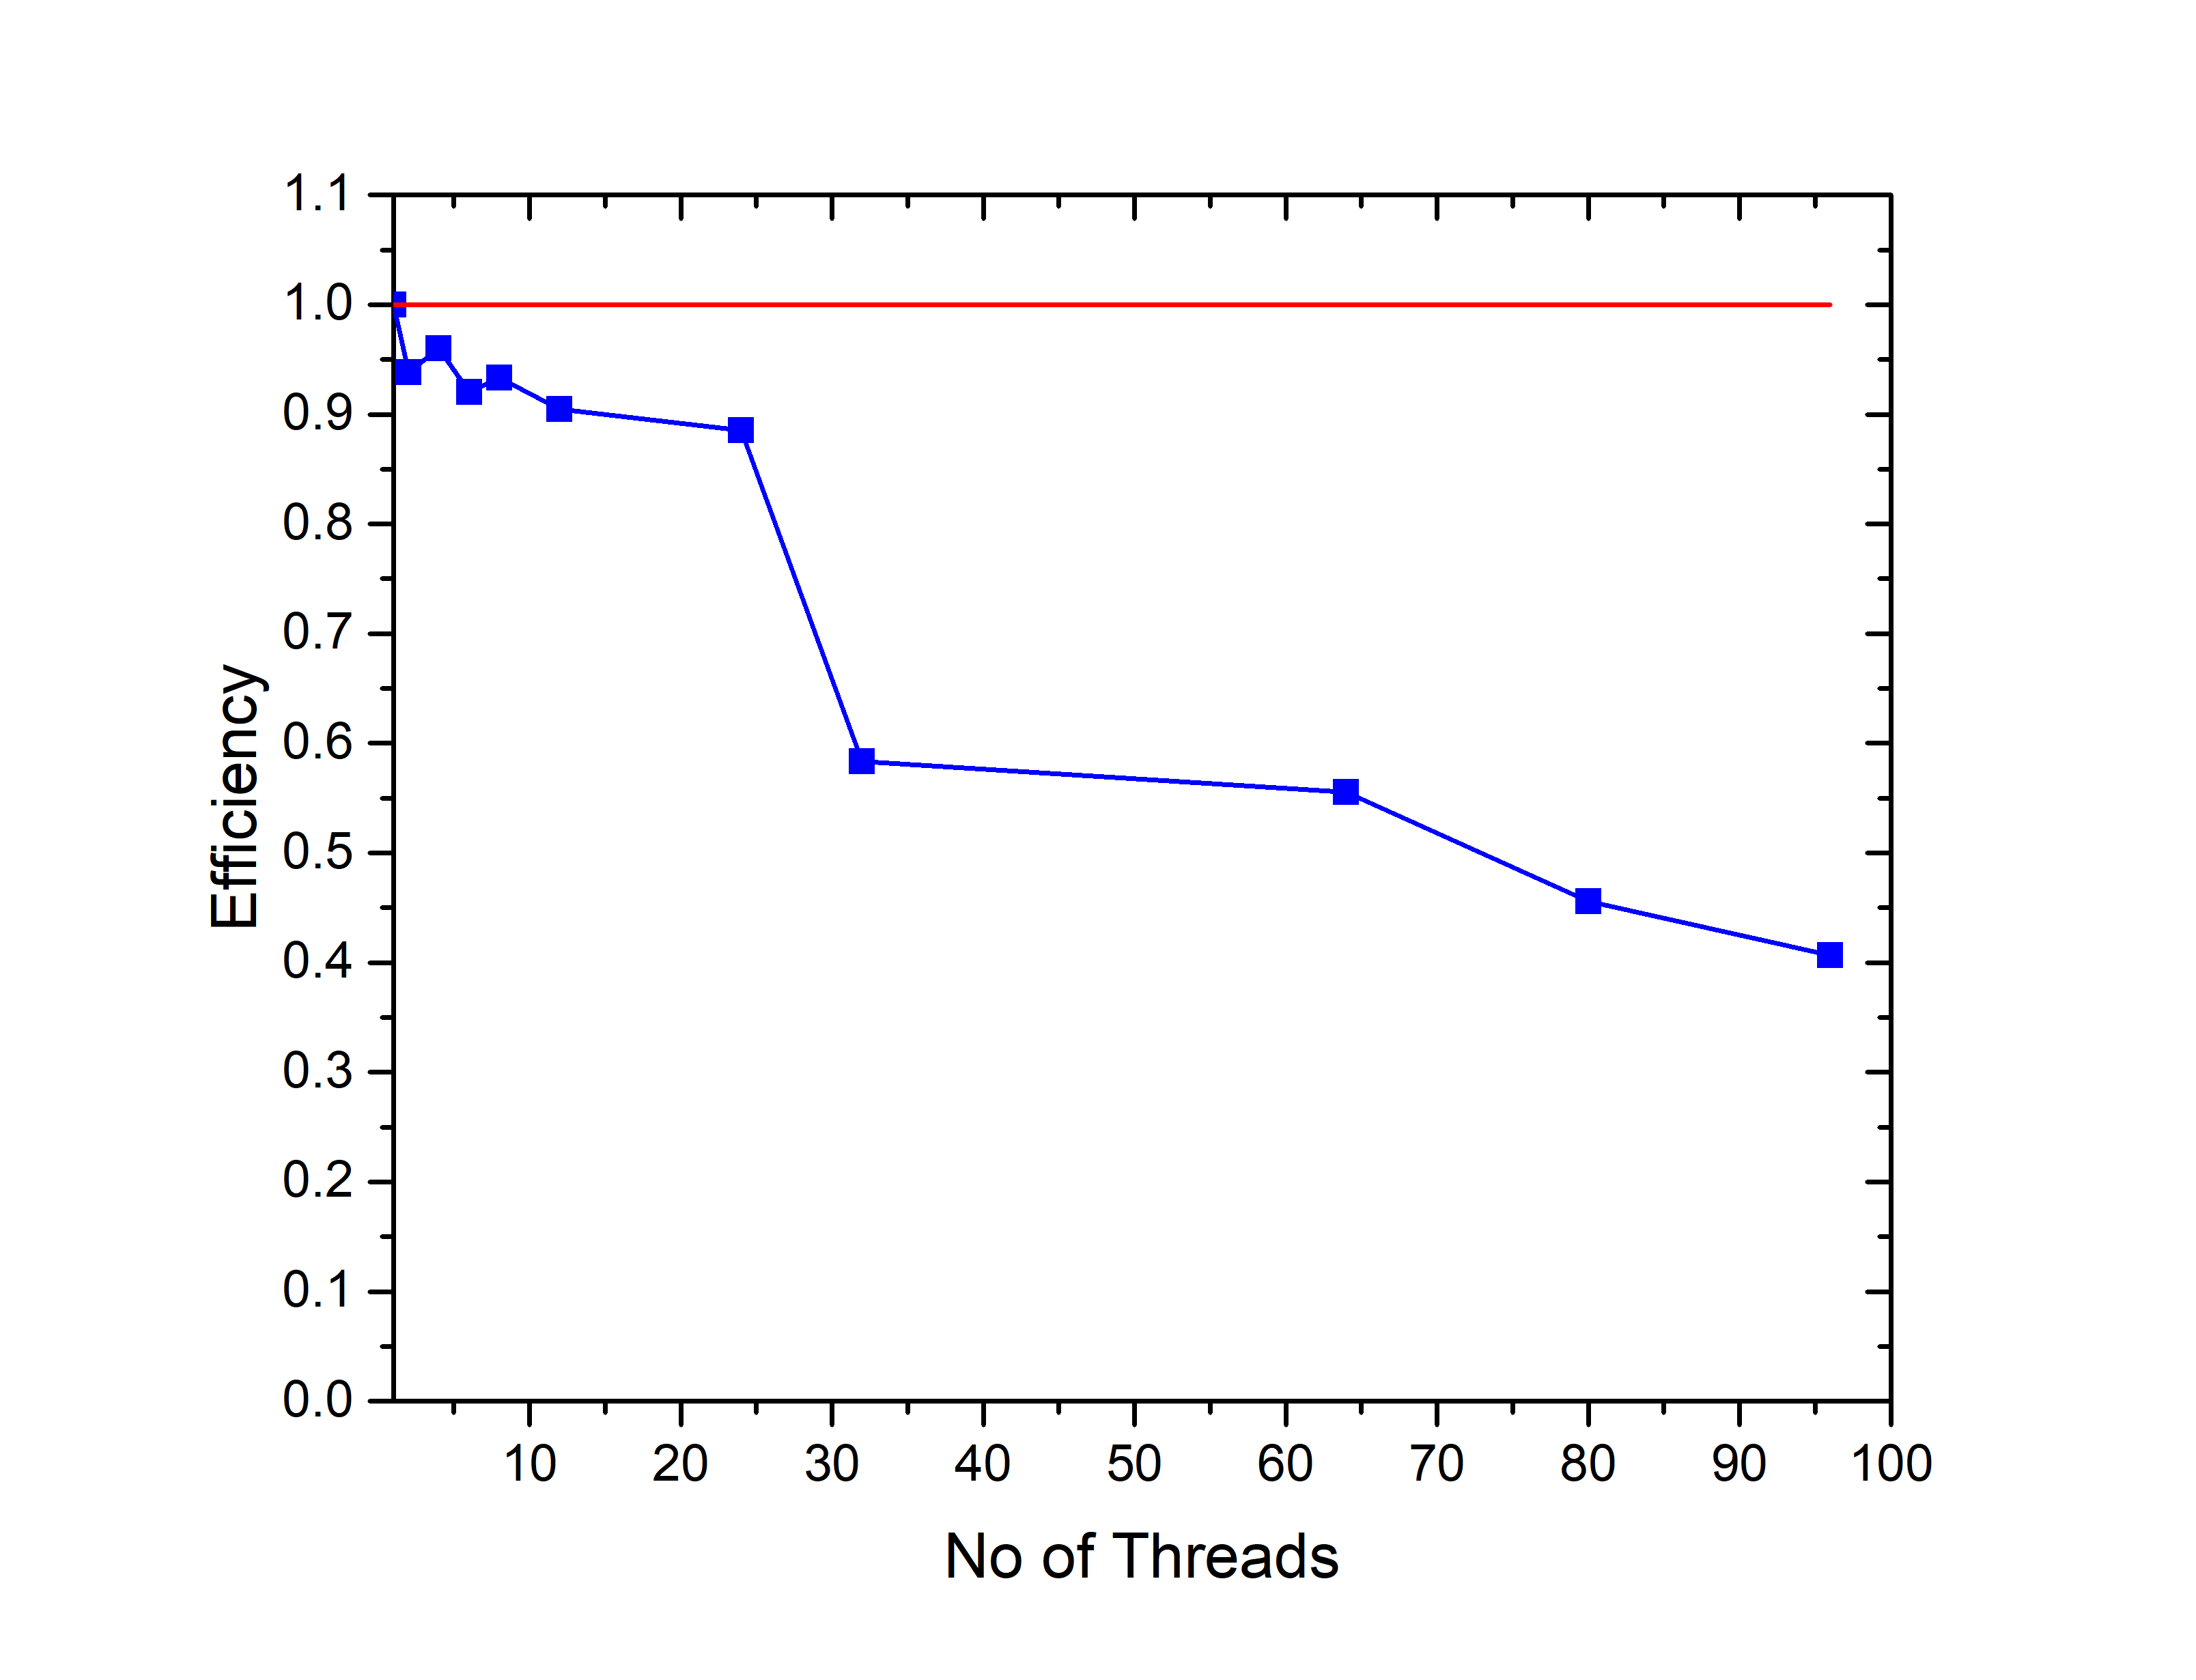
\includegraphics[width=0.5\textwidth]{WeakS.png}
  \caption{Figure of Weak Scaling}
  \label{figWS}
\end{figure}
\subsubsection{e}
Include in your tar archive your commented source code and a graphical rendering of your results. 
\subsection{Tutorial: Programming in C}
\subsubsection{Setting up your programming environment}
The gcc version of my local laptop is shown in Figure~\ref{figGCC}. 
\begin{figure}[h]
  \centering
  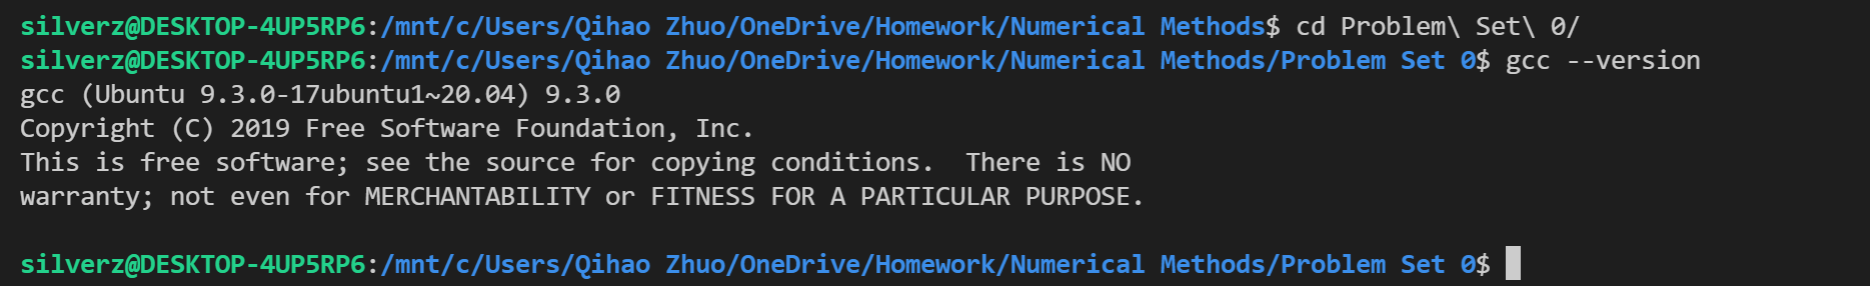
\includegraphics[width=0.8\textwidth]{gccEnviron.png}
  \caption{GCC Vsersion}
  \label{figGCC}
\end{figure}

\subsubsection{Writing a "hello world" program in C}
The output of \textbf{/.hello} in terminal is shown below. 
{\small\begin{framed}
\begin{lstlisting}[language=bash]
  Hello world 0 0.000
  Hello world 1 2.500
  Hello world 2 5.000
  Hello world 3 7.500
  Hello world 4 10.000
  Hello world 5 12.500
  Hello world 6 15.000
  Hello world 7 17.500
  Hello world 8 20.000
  Hello world 9 22.500
  10 22.500
  9 20.000
  8 17.500
  7 15.000
  6 12.500
  5 10.000
  4 7.500
  3 5.000
  2 2.500
  1 0.000
  \end{lstlisting}
\end{framed}}

\subsection{Parrallelizing your code using OpenMP}
The output of \textbf{/.hello\_omp} in terminal is shown below. 
{\small\begin{framed}
  \begin{lstlisting}[language=bash]
    Hello from thread 2, i=6, data=15.000
    Hello from thread 2, i=7, data=17.500
    Number of threads is 4
    Hello from thread 0, i=0, data=0.000
    Hello from thread 0, i=1, data=2.500
    Hello from thread 0, i=2, data=5.000
    Hello from thread 1, i=3, data=7.500
    Hello from thread 1, i=4, data=10.000
    Hello from thread 1, i=5, data=12.500
    Hello from thread 3, i=8, data=20.000
    Hello from thread 3, i=9, data=22.500
    End of parallel region
    tid=32685, 0 0.000
    tid=32685, 1 2.500
    tid=32685, 2 5.000
    tid=32685, 3 7.500
    tid=32685, 4 10.000
    tid=32685, 5 12.500
    tid=32685, 6 15.000
    tid=32685, 7 17.500
    tid=32685, 8 20.000
    tid=32685, 9 22.500
    \end{lstlisting}
  \end{framed}}
\end{document}
